\documentclass[titlepage, 12pt, leqno]{article}

% -------------------------------------------------- %
% -------------------- PACKAGES -------------------- %
% -------------------------------------------------- %
\usepackage{import}
\usepackage{pdfpages}
\usepackage{mathtools}
\usepackage{transparent}
\usepackage{enumitem}
\usepackage{xcolor}
\usepackage{tcolorbox}
\usepackage{amsmath}
\usepackage{placeins}
\usepackage{amssymb}
\usepackage{parskip}
\usepackage{bbm}
\usepackage[margin = 1in]{geometry}
\tcbuselibrary{breakable}
\tcbset{breakable = true}


% -------------------------------------------------- %
% -------------- CUSTOM ENVIRONMENTS --------------- %
% -------------------------------------------------- %
\newtcolorbox{note}{colback=black!5!white,
                          colframe=black!55!white,
                          fonttitle=\bfseries,title=Note}

\newtcolorbox{ex}{colback=blue!5!white,
                          colframe=blue!55!white,
                          fonttitle=\bfseries,title=Example}

\newtcolorbox{definition}{colback=red!5!white,
                          colframe=red!55!white,
                          fonttitle=\bfseries,title=Definition}


% -------------------------------------------------- %
% ------------------- COMMANDS --------------------- %
% -------------------------------------------------- %
% Brackets, braces, etc. 
\newcommand{\abs}[1]{\lvert #1 \rvert}
\newcommand{\bigabs}[1]{\Bigl \lvert #1 \Bigr \rvert}
\newcommand{\bigbracket}[1]{\Bigl [ #1 \Bigr ]}
\newcommand{\bigparen}[1]{\Bigl ( #1 \Bigr )}
\newcommand{\ceil}[1]{\lceil #1 \rceil}
\newcommand{\floor}[1]{\lfloor #1 \rfloor}
\newcommand{\norm}[1]{\| #1 \|}
\newcommand{\bignorm}[1]{\Bigl \| #1 \Bigr \| #1}
\newcommand{\inner}[1]{\langle #1 \rangle}
\newcommand{\set}[1]{{ #1 }}


% -------------------------------------------------- %
% -------------------- SETUP ----------------------- %
% -------------------------------------------------- %
\title{\Huge{The Social and Political Effects of Misinformation Consumption}}
\author{\large{Mitch Harrison}}
\date{\today}   
\begin{document}
\setlength{\parskip}{1\baselineskip}
\setlength{\parindent}{15pt}
\maketitle
\tableofcontents
\newpage


% -------------------------------------------------- %
% --------------------- BODY ----------------------- %
% -------------------------------------------------- %
\section{Abstract}
Misinformation is an epidemic in the United States, and the age of "alternative facts" is still in its infancy. Therefore, the long-term social effects of misinformation are challenging to study at this early stage. In this piece, I seek to model the impact of misinformation on social relationships among regular media consumers to help predict the long-range social impacts of misinformation consumption. I create a network graph in which nodes are either producers (i.e., media companies that output information) or consumers (i.e., viewers/readers of information). Producers are connected to the consumers of their content with non-directed edges. Additionally, consumers are connected to other consumers, representing social connections between citizens, either in-person or online. This model shows that, over time, media sources that output misinformation do not suffer a lack of viewership. While they may lose the trust of some consumers, enough stay dedicated to keep their business afloat while driving partisan wedges between most consumers of different parties. Additionally, between-consumer relationships suffer an increasing lack of political diversity and, for some consumers, shrink in absolute number, even as consumers of misinformation become closer to one another.

\pagebreak
\section{Introduction}
In 2022, Merriam-Webster's word of the year was "gaslighting" [4]. In 2023, it was "authentic" [5]. The 2020s have already been defined by the battle between truth and misinformation. It is too early to tell the long-term impact of the age of "alternative facts," but modeling the social implications of misinformation may help brace readers for that impact on themselves or their loved ones. 

The impact of misinformation may not be purely social. While cross-politics connections are healthy for a functioning democracy, what may be even more damaging is increased polarization along the lines of what the US and much of the world are already experiencing [6,9]. The combination of the social closing off of opposing political views and increased political polarization make for a dangerous cocktail that could poison democracy worldwide. Misinformation may be a vital ingredient of that cocktail.

In this report, I hope to analyze the long-term effects of misinformation consumption on both consumers and non-consumers of such misinformation to help measure possible sociopolitical outcomes of "alternative facts."

\pagebreak
\section{Literature Review}
This study builds a social network represented by a graph network to simulate the social and political connections between users and media sources and between users and other users (the latter relationship is classified as "friends"). But friendship diversity is non-uniform across the political spectrum. Pew Research investigated the realities of friendship in the United States and found that (perhaps surprisingly) most partisan citizens have at least "a few" close friends of the opposing political party [2]. In my graph network (with only two media sources and 18 consumers), I use this data to decide how many cross-party friendships the model begins with.

Fortunately, Pew also investigated not just the partisan diversity of American friendship but the total number of friends that Americans have. Most Americans report having four or more close friends, and nearly 40\% report having five or more [2]. However, because my network's population is so much smaller than the American population, I shrink the absolute number of friends for each node to account for the smaller scale. One could read this change as a "friendship" counting as a more significant trend in total friendship between nodes representing populations of people, not individuals. The result of these Pew findings is a rough approximation of social relationships between partisan Americans who consume regular news media.

However, consumers are not the only biased members of society. Media sources are also intensely biased (some more than others), and those biases may drive one another into a polarizing spiral. AllSides Media Bias Ratings show these media biases [1]. Because my model is a simplified network, I've grouped all non-centrist media sources into two nodes: the "red" media source (called a "producer" from hereon) and the "blue" producer, representing conservative and liberal media, respectively. 

While many Americans consume diverse media [8], for ease of computation, I have assigned all consumers exclusively to producers of their own color, and only the conservative producer outputs misinformation. This decision is arbitrary, and the simulation functions with either party being assigned a non-zero misinformation rate.

\pagebreak
\section{Methodology}
To investigate the role of misinformation on political polarization and social stability, I construct a graph network in which nodes represent either producers (i.e., media sources) or consumers. Edges from producers to consumers represent a consumer getting political news from that producer. These producer/consumer connections are always of the same political leaning. Other edges are consumer-to-consumer, meaning social relationships between two human actors (hereon called a "friendship"). This friendship could be online or in-person. Crucially, because the number of consumers is so low compared to real-world media consumption, these nodes are better understood as representing larger populations of people, all of whom consume regular political news from sources of their own partisan leanings. Note that edge weights will grow and shrink over time and be deleted if they grow too weak.

Producers and consumers have both shared and unique characteristics. Both consumers and producers have a "party." That is, they both are colored red if they have a conservative lean and blue if they have a liberal lean. However, unlike producers, consumers have a political score representing how partisan they are. This political score is centered on zero and grows increasingly positive as consumers become more conservative and increasingly negative as they become more liberal. Producers only have a party but no political score.

Producers also have a misinformation rate, which decides how often they output misinformation. While a simple binary classifier of "misinformation" or "not misinformation" is often impossible to obtain, representing media in this way aids in exploring the impact of misinformation, even if it is less rigidly defined than a simple 1 or 0.

At each iteration of the model, both media sources output information and consumers react to this new information. If the information the producer sends is not misinformation, a slight positive change in trust in that source occurs (represented by an increased edge weight from a consumer to that producer). If it is misinformation, consumers have a significant spike in trust if they are sufficiently partisan in that producer's direction and a drop in trust if not. The conservative media source has a misinformation rate of 0.5, which is much more extreme than is likely to be observed in the real world but helps speed up the model to arrive at equilibria faster.

After each iteration's media is consumed by all consumers, political scores are shifted for each of them. If a consumer has friends of a different party, their partisan lean changes much more slowly. If their friends are entirely of the same party but none of those friends are highly partisan, they polarize slightly faster. Finally, if all of a consumer's friends have a strong partisan lean, they lack friends of a different party, and they place large trust in misinformation, they polarize even faster.

After each polarization score is calculated, friendships change. For each consumer-to-consumer friendship, the strength of the friendship (represented by edge weight) goes up if they are similarly politically aligned or consume the same media and down if they have a strong distrust of the press that their friends consume. However, to offset the obvious polarizing factor that an "if opposite party, break friendship" algorithm would cause, consumers also randomly generate new friendships at each iteration. Those new friendships have a moderate starting weight and can often survive and bring down the partisan lean of the consumers involved.

What results is a simplified graph-network model of social relationships among consumers of political media, one of which produces misinformation. 

\pagebreak
\section{Data Presentation}
At iteration zero (i.e., before any information had been output by any producer), there was some partisan grouping of friendships but a diversity approximating Pew's findings. However, there were very few cross-party friendships after 20 iterations (recall that a misinformation rate of 0.5 was used to speed up this process). Figures 1 and 2 show the graph network at iterations 0 and 20, respectively. Notice that after consuming misinformation, only two cross-party friendships remain. While this is especially low among other attempted runs, it is not uniquely low. Most runs produced a final number of cross-party friendships between two and four.

\begin{figure}[ht]
    \centering
    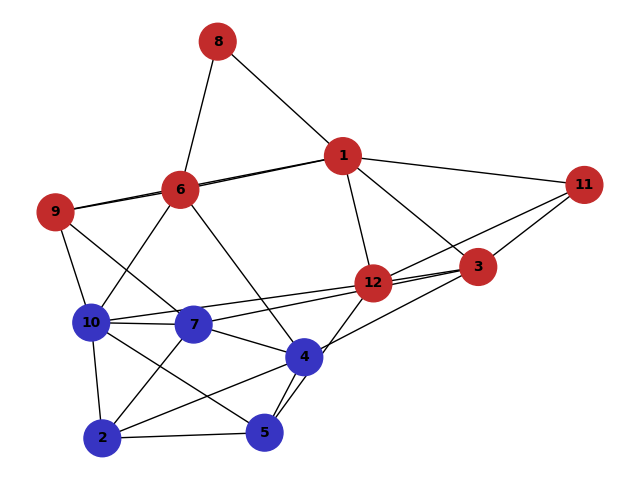
\includegraphics[width=0.8\textwidth]{../plots/graph_iter0.png}
    \caption{Starting graph network}
\end{figure}

\begin{figure}[ht]
    \centering
    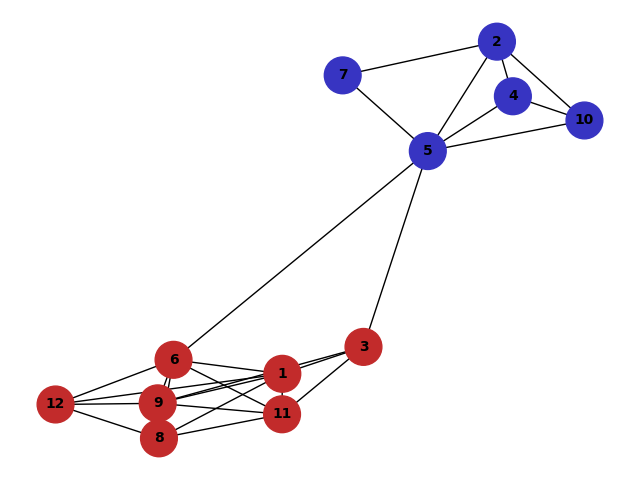
\includegraphics[width=0.8\textwidth]{../plots/graph_iter21.png}
    \caption{Final graph network}
\end{figure}


These visual representations hold up numerically. Interestingly, the network shows that even though these partisan islands form, consumers of misinformation ultimately end up more socially connected, not less. This may speak to a phenomenon that brings consumers of misinformation together around a shared distrust of more truthful media, which, in their view, distorts reality instead of reporting it fairly. We see a similar phenomenon among those who joined anti-"fake news" social media pages during the Trump era. Figure 3 shows this effect as a distribution of the number of friends by party at iterations zero and 20.

\begin{figure}[ht]
    \centering
    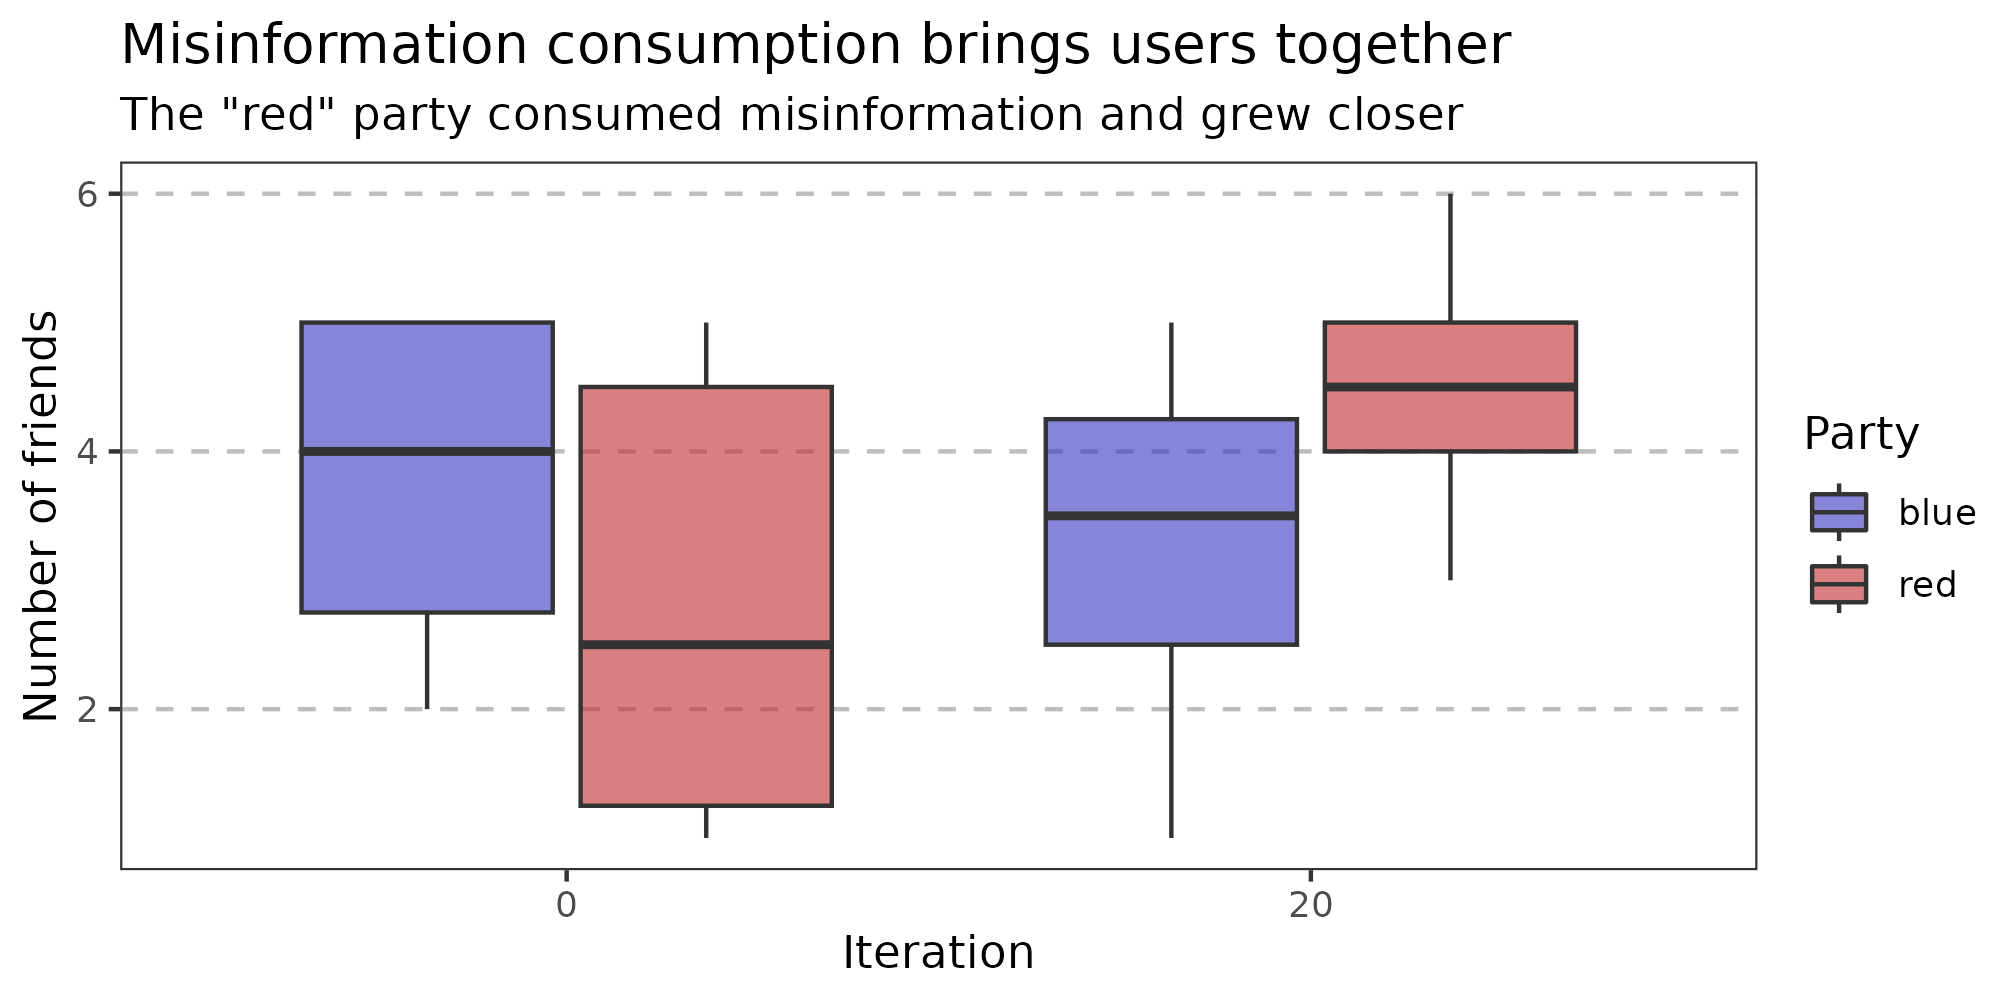
\includegraphics[width=0.6\textwidth]{../plots/nfriends_change.png}
    \caption{Number of friends change by party}
\end{figure}

\begin{figure}[ht]
    \centering
    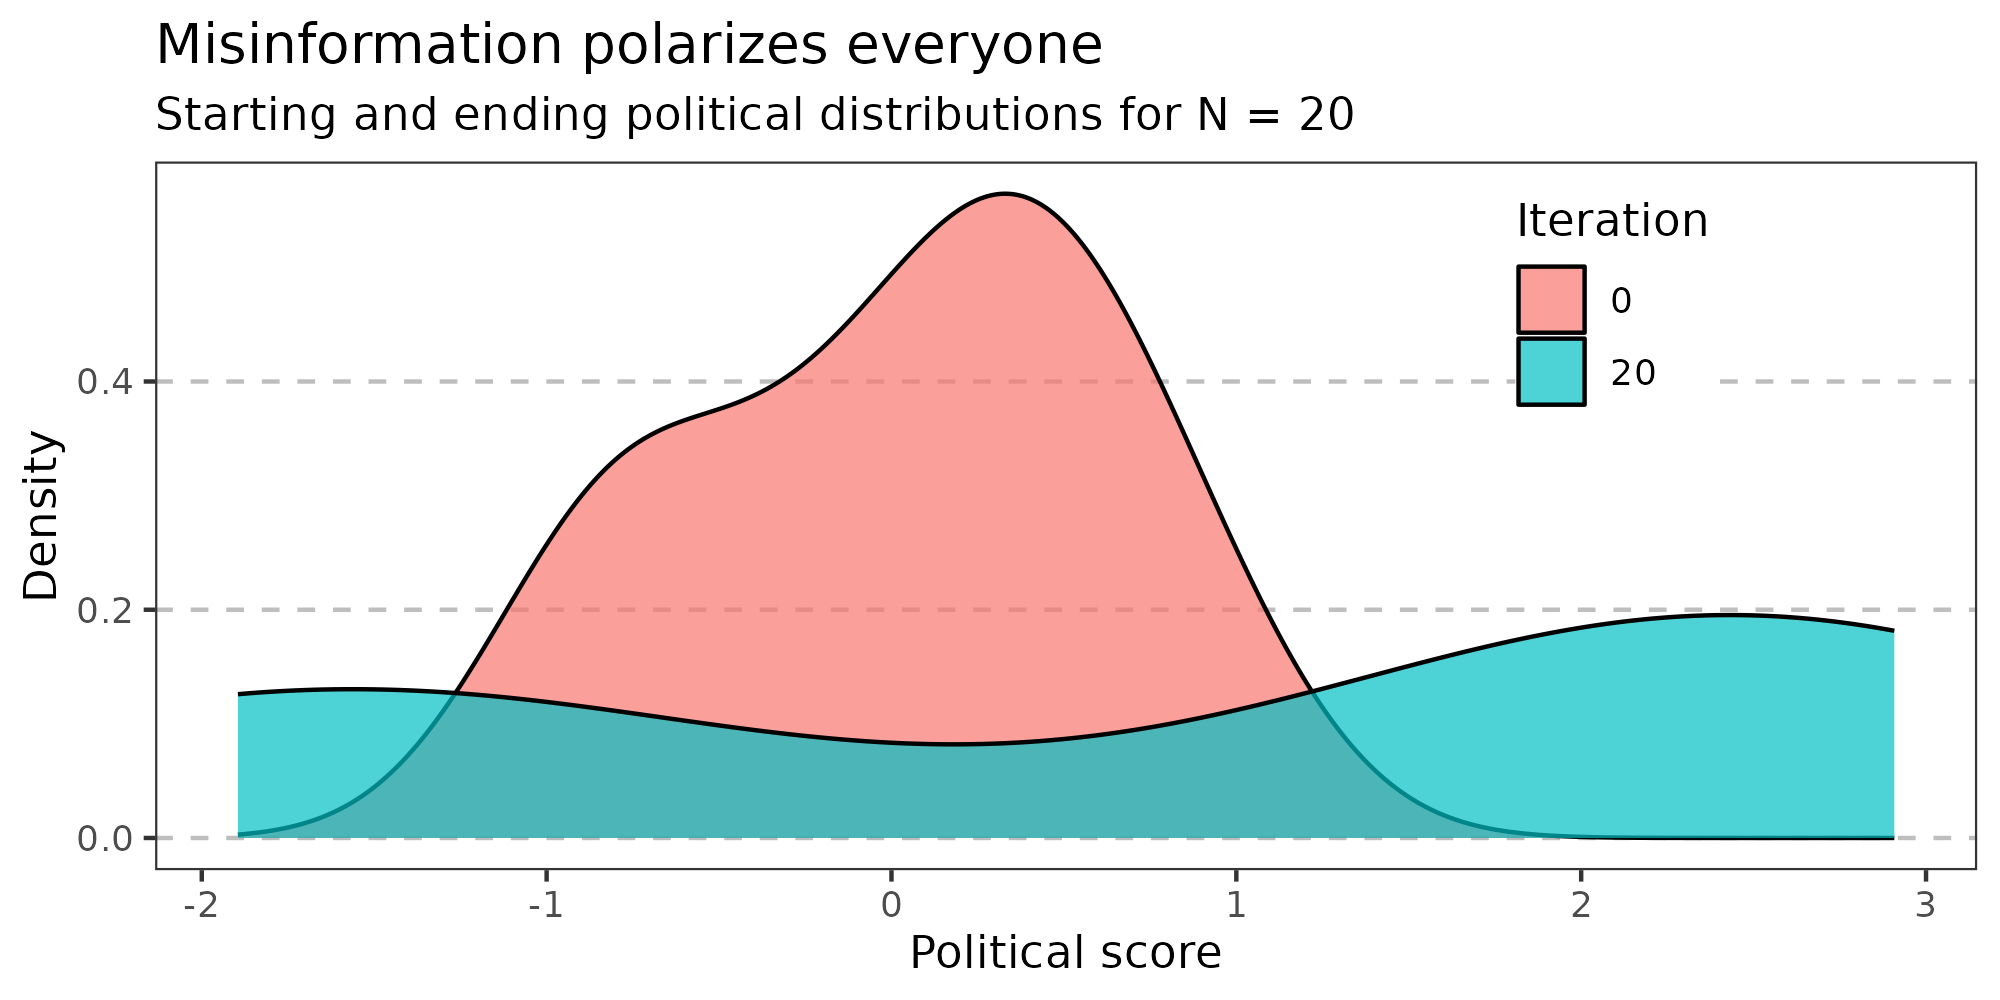
\includegraphics[width=0.6\textwidth]{../plots/polscore_change.png}
    \caption{caption}
\end{figure}

Finally, and perhaps most importantly, the network allows us to explore the polarizing effect of misinformation. Figure 4 shows the population's starting (in red) and final (in blue) political distributions. It is clear that the mode of the score density is between 0 and 0.5 at the start of the simulation. But after its conclusion, the middle has fallen out. Perhaps unsurprisingly, the consumers of misinformation become slightly more partisan in the positive direction than non-misinformation consumers do in the negative direction. However, non-misinformation consumers were not immune to the polarization effect. As distrust for each of the opposing sides builds, they push each other in the opposite direction, even when only one party is consuming misinformation. Figure 5 shows the variance of these starting and ending political distributions by party. While the variance remained relatively consistent, the mean political scores shifted in both extremes, as seen in Figure 4. We also see the apparent shift further from 0 by those who consume misinformation (in red).

\begin{figure}[ht]
    \centering
    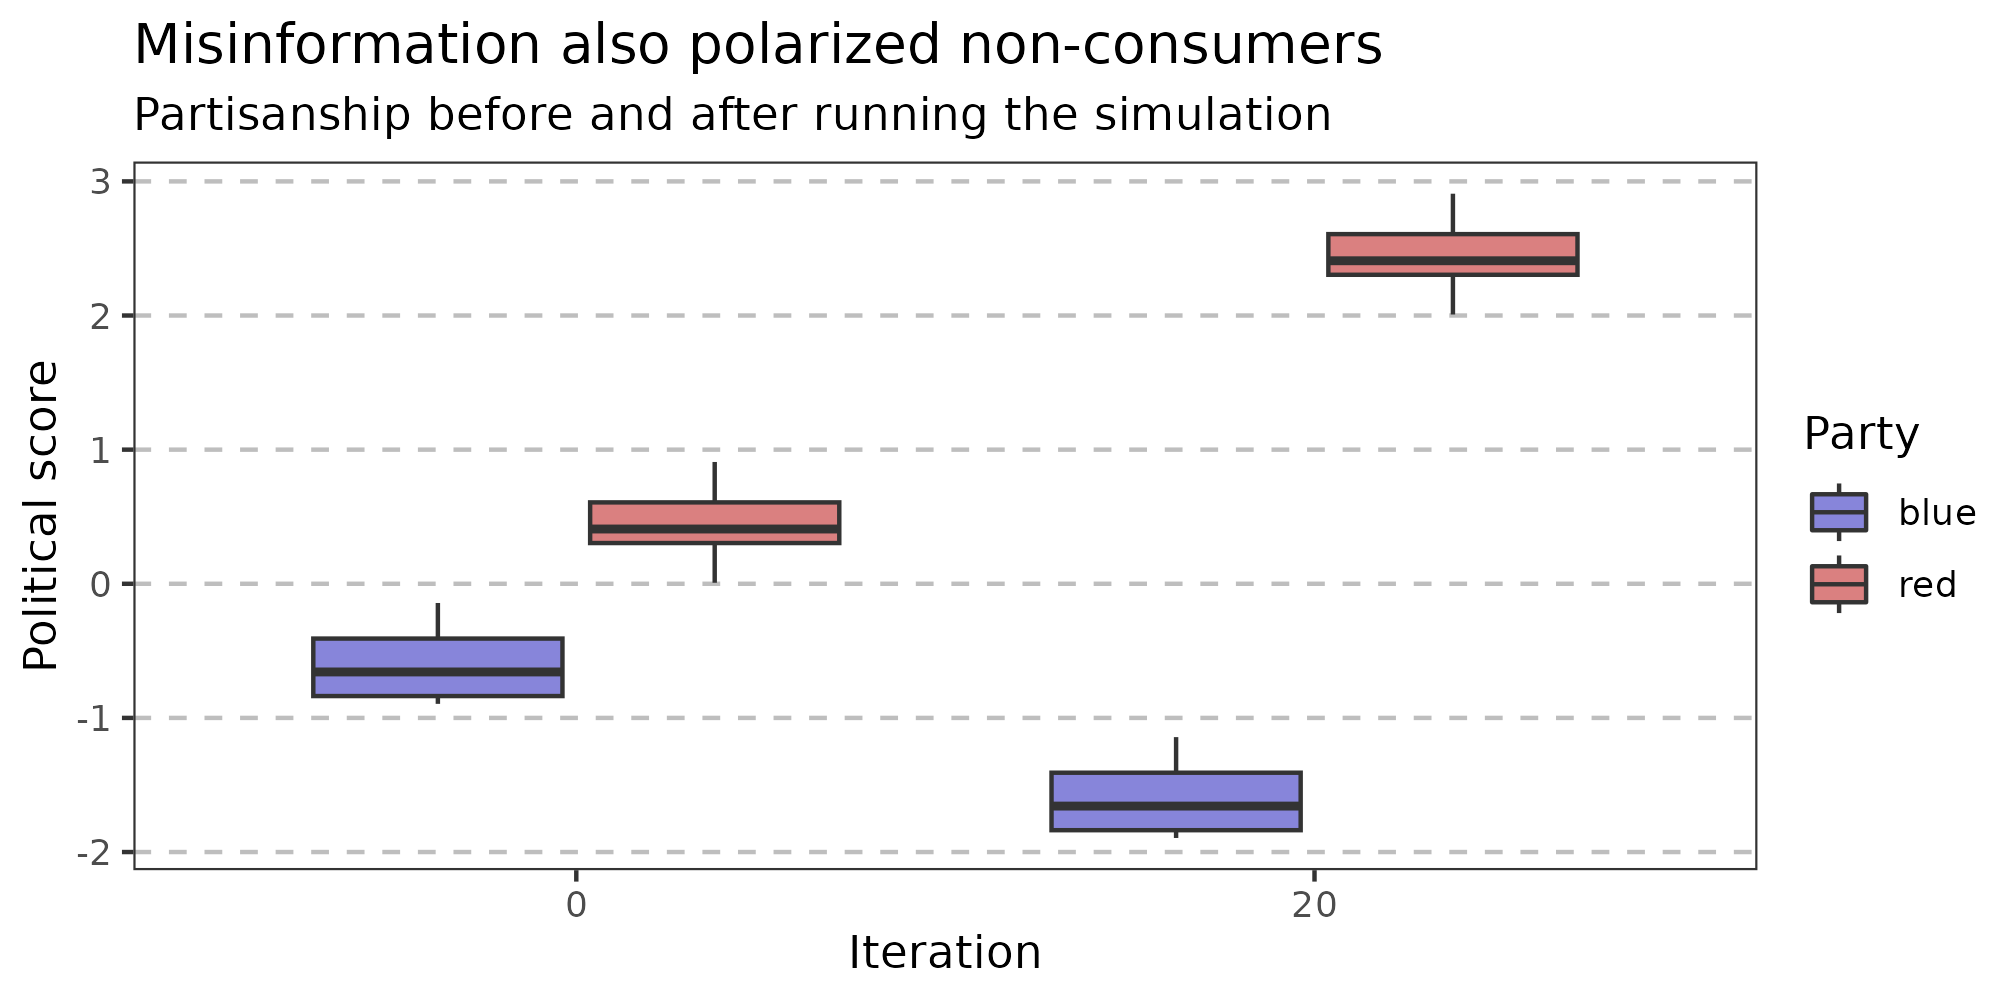
\includegraphics[width=0.6\textwidth]{../plots/polscore_change_box.png}
    \caption{Political score changes by party}
\end{figure}

\FloatBarrier
\pagebreak
\section{Conclusion}
Misinformation appears to be toxic to both diversity in social relationships and to political polarization. However, this effect is not linear. In fact, consumers of misinformation do not appear to be alone on their social island, unquestioningly consuming media and becoming increasingly socially toxic. The effect is quite the opposite: misinformation consumers have strong social ties and large social networks; they save their social trust for those among their in-group, as do those who do not consume such misinformation.

The effect on polarization is also surprising. While one would likely expect that misinformation consumers would become polarized by their media (as the model shows), those who consume accurate media also show a polarization effect as trust for the opposing side shrinks. While this effect is lessened by consuming more accurate media, it is certainly non-zero.

Finally, one could hope for a media ecosystem and political culture that punishes misinformation producers by shrinking their viewership/readership. However, that is not the case. Viewership among the producers of misinformation stayed strong, and a community of interconnected consumers formed, keeping each other polarized and connected to that same source.

\subsection{Future research}
Despite the answers provided by this simulation, much more research is needed in this field. Most importantly, there is no widely accepted standard for classifying misinformation/disinformation. This absence is understandable, especially with the comparatively new floodgate of online misinformation that has opened in the past several years and the difficulty of such classification. Although research is being done in that space, assigning a "misinformation rate" to a simulated media source is a dramatic oversimplification of the nuances of propaganda and misinformation. 

\pagebreak
\section*{References}
\begin{enumerate}[label={[\arabic*]}]
    \item \textit{Allsides Media Bias Chart}. AllSides. (2023, October 20).
        https://www.allsides.com/ media-bias/media-bias-chart 
    \item Goddard, I. (2023, October 12). \textit{What does friendship look like 
        in America?} Pew Research Center. https://www.pewresearch.org/
        short-reads/2023/10/12/what-does-friendship-look-like-in-america/ 
    \item Granados, N. (2023, January 17). Media trends: \textit{Why 
        misinformation is here to stay}. Forbes. https://www.forbes.com/sites/
        nelsongranados/2023/01/12/
        media-trends-why-misinformation-is-here-to-stay/ 
    \item Merriam-Webster. (n.d.-a). \textit{Word of the year 2022}. Merriam-
        Webster. https://www. merriam-webster.com/wordplay/word-of-the-year-2022 
    \item Merriam-Webster. (n.d.-b). \textit{Word of the year 2023}. Merriam-
        Webster. https://www. merriam-webster.com/wordplay/word-of-the-year 
    \item Pew Research Center. (2014, June 12). \textit{Political polarization 
        in the American public}. Pew Research Center - U.S. Politics \& Policy.
        https://www.pewresearch.org/politics/ 2014/06/12/political-polarization-
        in-the-american-public/ 
    \item Pew Research Center. (2016, June 22). \textit{3. partisan 
        environments, views of political conversations and disagreements}. Pew 
        Research Center - U.S. Politics \& Policy. https://www.pewresearch.org/
        politics/2016/06/22/3-partisan-environments-views-of -political-
        conversations-and-disagreements/ 
    \item Pew Research Center. (2020, January 24). \textit{2. Americans are 
        divided by party in the sources they turn to for Political News}. Pew
        Research Center’s Journalism Project. https://www.pewresearch.org/
        journalism/2020/01/24/americans-are-divided-by-\\party-in-the-sources-
        they-turn-to-for-political-news/ 
    \item The rise in political violence in the United States and damage to
        our ... (n.d.). https://carnegieendowment.org/2022/03/31/rise-in-
        political-violence-in-united-\\states-and-damage-to-our-democracy-pub-
        87584 
\end{enumerate}

\end{document}
